\pling\ is a portfolio-based SAT solver... [[Short explanation of plingeling]]

\subsection{Modified \pling}
\label{sec:modifiedpling}


One of the advantages we assume of parallel computing is that the more
cores we add, the better performance we will obtain. This should be
also true for \pling, since the only difference of adding more threads
(assuming we have one thread per core) is that we will have a greater
variety of solver strategies trying to solve the same problem, and
also some logical clause sharing among threads. These are all valid
assumptions in theory, but empirical results on multicore shared
memory computers also show us that increasing the number of threads
also carries a considerable decrease in performance for portfolio
solvers like {\tt plingeling} due to cache misses. In what follows, we
explain this in detail.

Multicore shared memory systems have their cores sharing the same last
level cache (LLC) memory. The last level cache size in modern machines
has a few megabytes and is usually not enough to hold all the data
required by a SAT instance. Therefore, there will be inevitably some
communication between the LLC and main memory. The time cost of
communication between the CPU and the LLC cache are much faster than
having to get data from main memory, so we would like to keep data
transfers from main memory to a bare minimum.

Portfolio SAT solvers which only share clauses logically have to keep
a complete database of clauses for each thread's use. So as we add
more threads, the solver has greater needs of memory, but because all
cores share the same LLC, all threads will have a lower chance of
finding their data in the LLC as we add more threads. In this
scenario, what we would expect to observe, as we have in our
experiments, is a considerable decrease in performance when adding
threads, simply because we incur in more LLC cache misses when the
amount of data to be manipulated by different threads increases. We
don't usually appreciate this negative performance impact in these
type of solvers, because different threads implement different SAT
solving strategies, so the solving time will mostly depend on the
fastest solving thread, shadowing the negative performance impact of
copying the clause database in each thread.

For experimentation puposes, we modifed \pling\ in such a way that
each thread did exactly the same search. For this, we initialized each
thread with the same ramdom seed, heuristic values and clause
database.  Furthermore, in order to keep them searching in the same
way, we disabled clause sharing between threads (which in \pling
corresponds to disabling the interchange of found units) and assure
that cleanup policies and algorithms were the same. In these
experiments, we would expect, theoretically, that adding more threads
would have no impact in the solving time, because all cores would be
making the exact same search with their own data. However, in
practice, we found that the performance decay of having ten threads
spread over ten cores ranged from about 21\% (1.21 times slower) to
200\% (3 times slower) of the total time one thread would take (Figure
\ref{fig:decay}). Possible reasons for this behavior may be due to
several factors in modern SMP architectures. However, sharing
resources (such as the caches, communication and/or synchronization,
or main memory) could be seen as the main suspects. To find out, we
ran another experiment where a \pling\ instance performing the same
search with four threads was executed on different physical CPU {\em
  chips} (rather than cores), and, to compare, we ran the same
experiment on four cores of the same CPU chip.

% Because each CPU has its own LLC
% cache, we would expect in this case to have equal performance when
% running one thread compared to running four threads, which is what was
% observed in our measures.

\begin{figure}
  \begin{center}
    \subfloat[on same
    chip]{\label{fig:4coressame}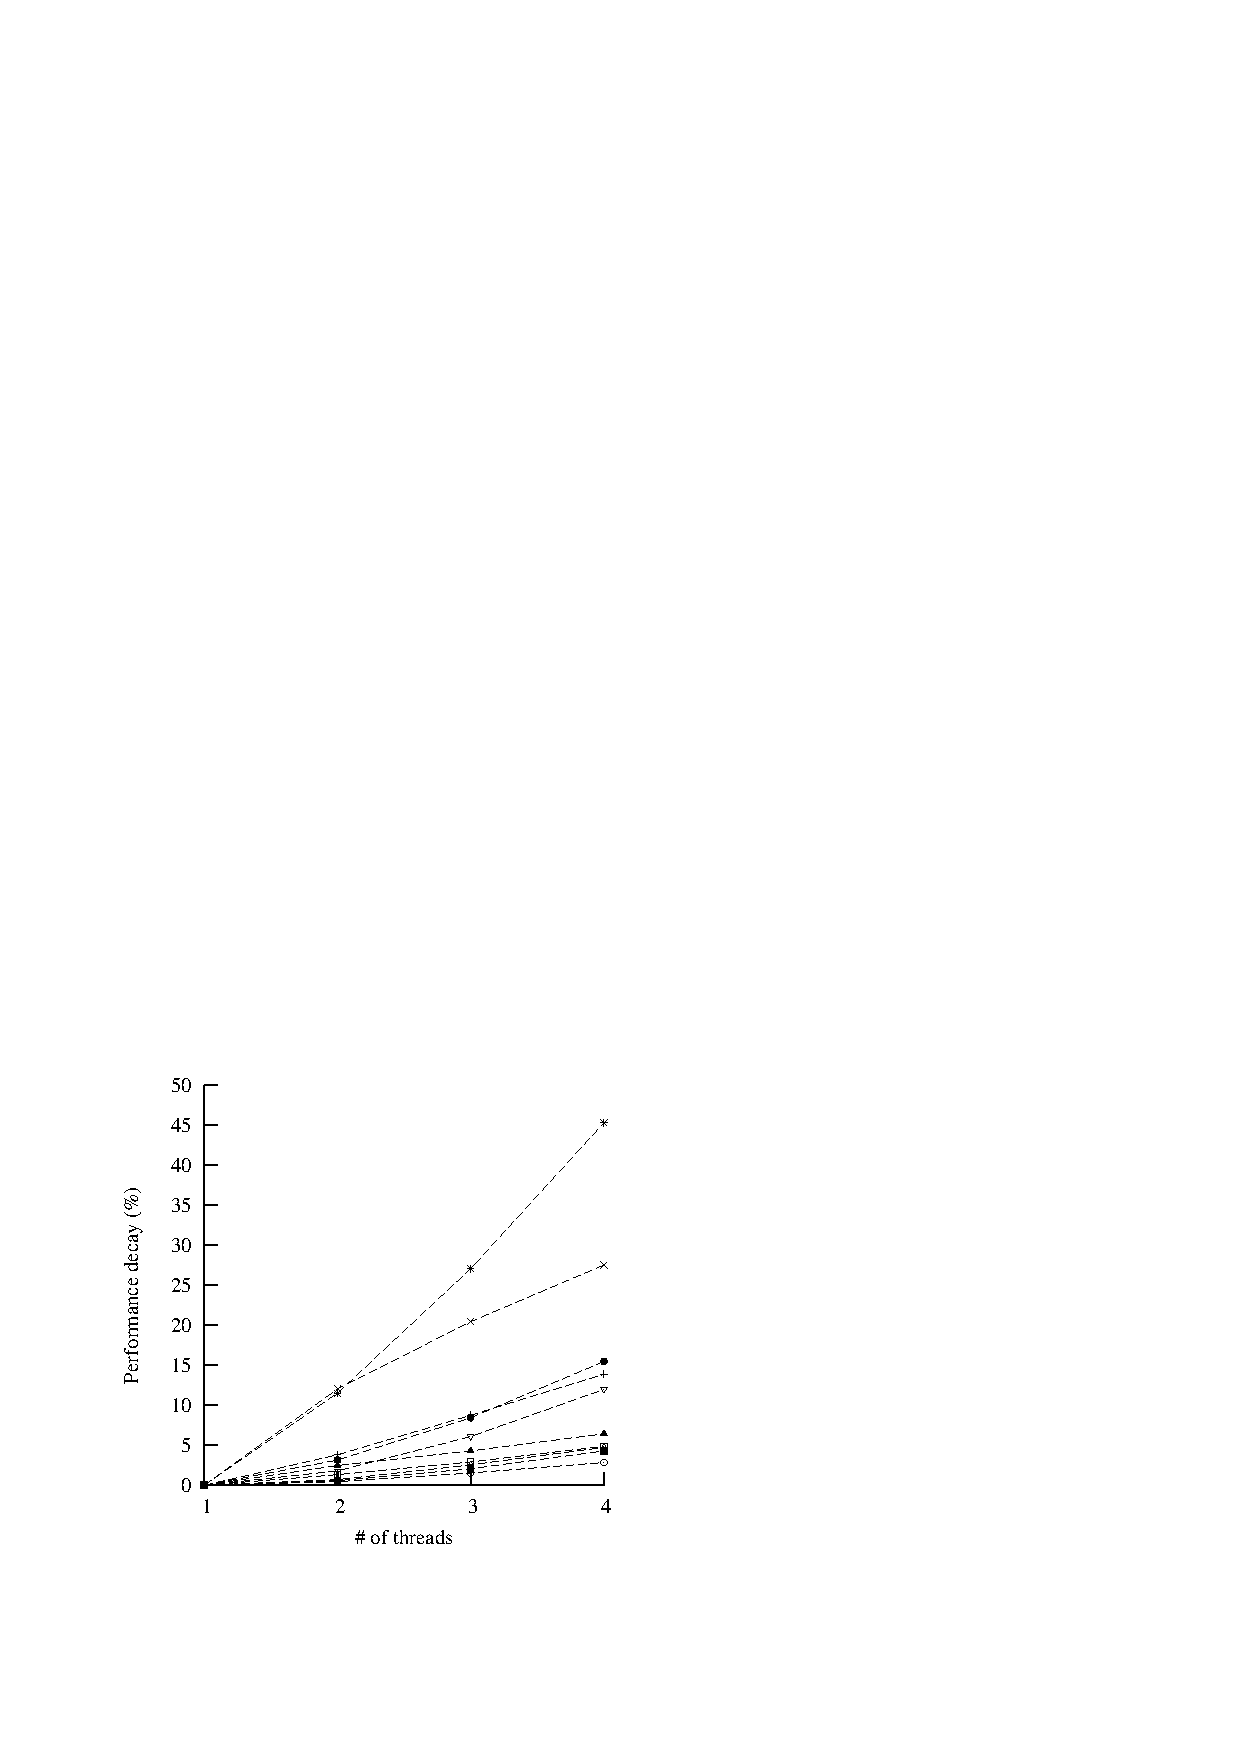
\includegraphics[bb=59 90 294 325,
      clip, width=0.5\textwidth]{plingeling_same_chip}} \subfloat[on
    different chips]{\label{fig:4coresdiff}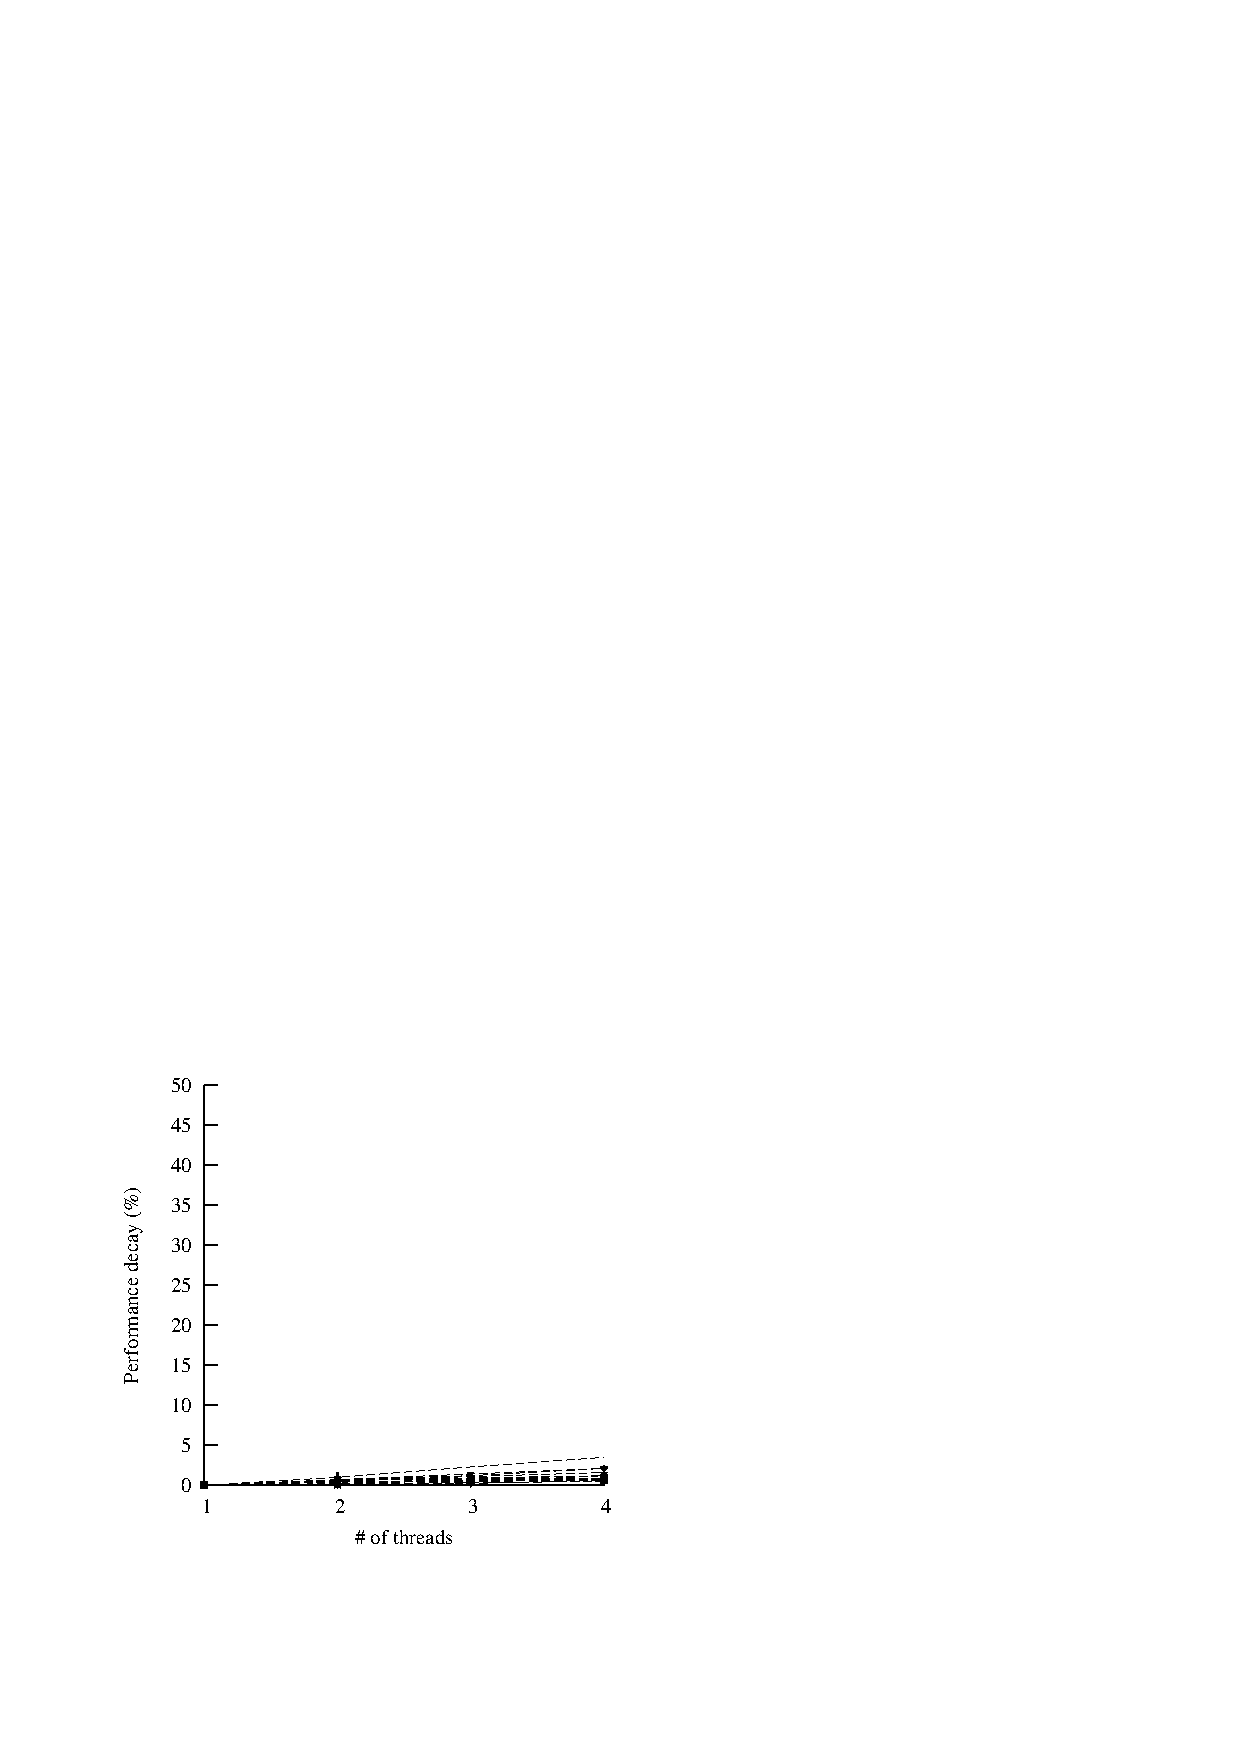
\includegraphics[bb=59
      90 294 325, clip,
      width=0.5\textwidth]{plingeling_different_chip}}
    \caption{Modified \pling\ performance decay}
  \end{center}
\end{figure} 

As can be seen, executing the solver on {\em different} CPU chips does
not impact performance, while executing it on the {\em same} CPU chip
incurs in a significant performance decay. According to the results
above, the only shared resource that could impact performance when run
in one chip is the LLC or Last Level Cache. To effectively measure the
involvement of the LLC, we used the {\tt perf}
tool\footnote{\url{perf.wiki.kernel.org}}. The {\tt perf} tool is a
hardware abstraction over hardware counters of the different CPU chips
integrated in the Linux kernel to access profiling information on
retired instructions, branch misprediction, and in particular for our
purposes counting percentage of cache misses over cache hits ({\em
  LLC-load-misses}). As Figure \ref{fig:LLCStats}) strongly suggests,
the performance decay observable in Figure \ref{fig:decay} is due to
several solving threads {\em thrashing} the cache and thus wasting
much more time retrieving their individual data from main memory than
their single-threaded counterparts.

\begin{figure}[h]
  \centering
  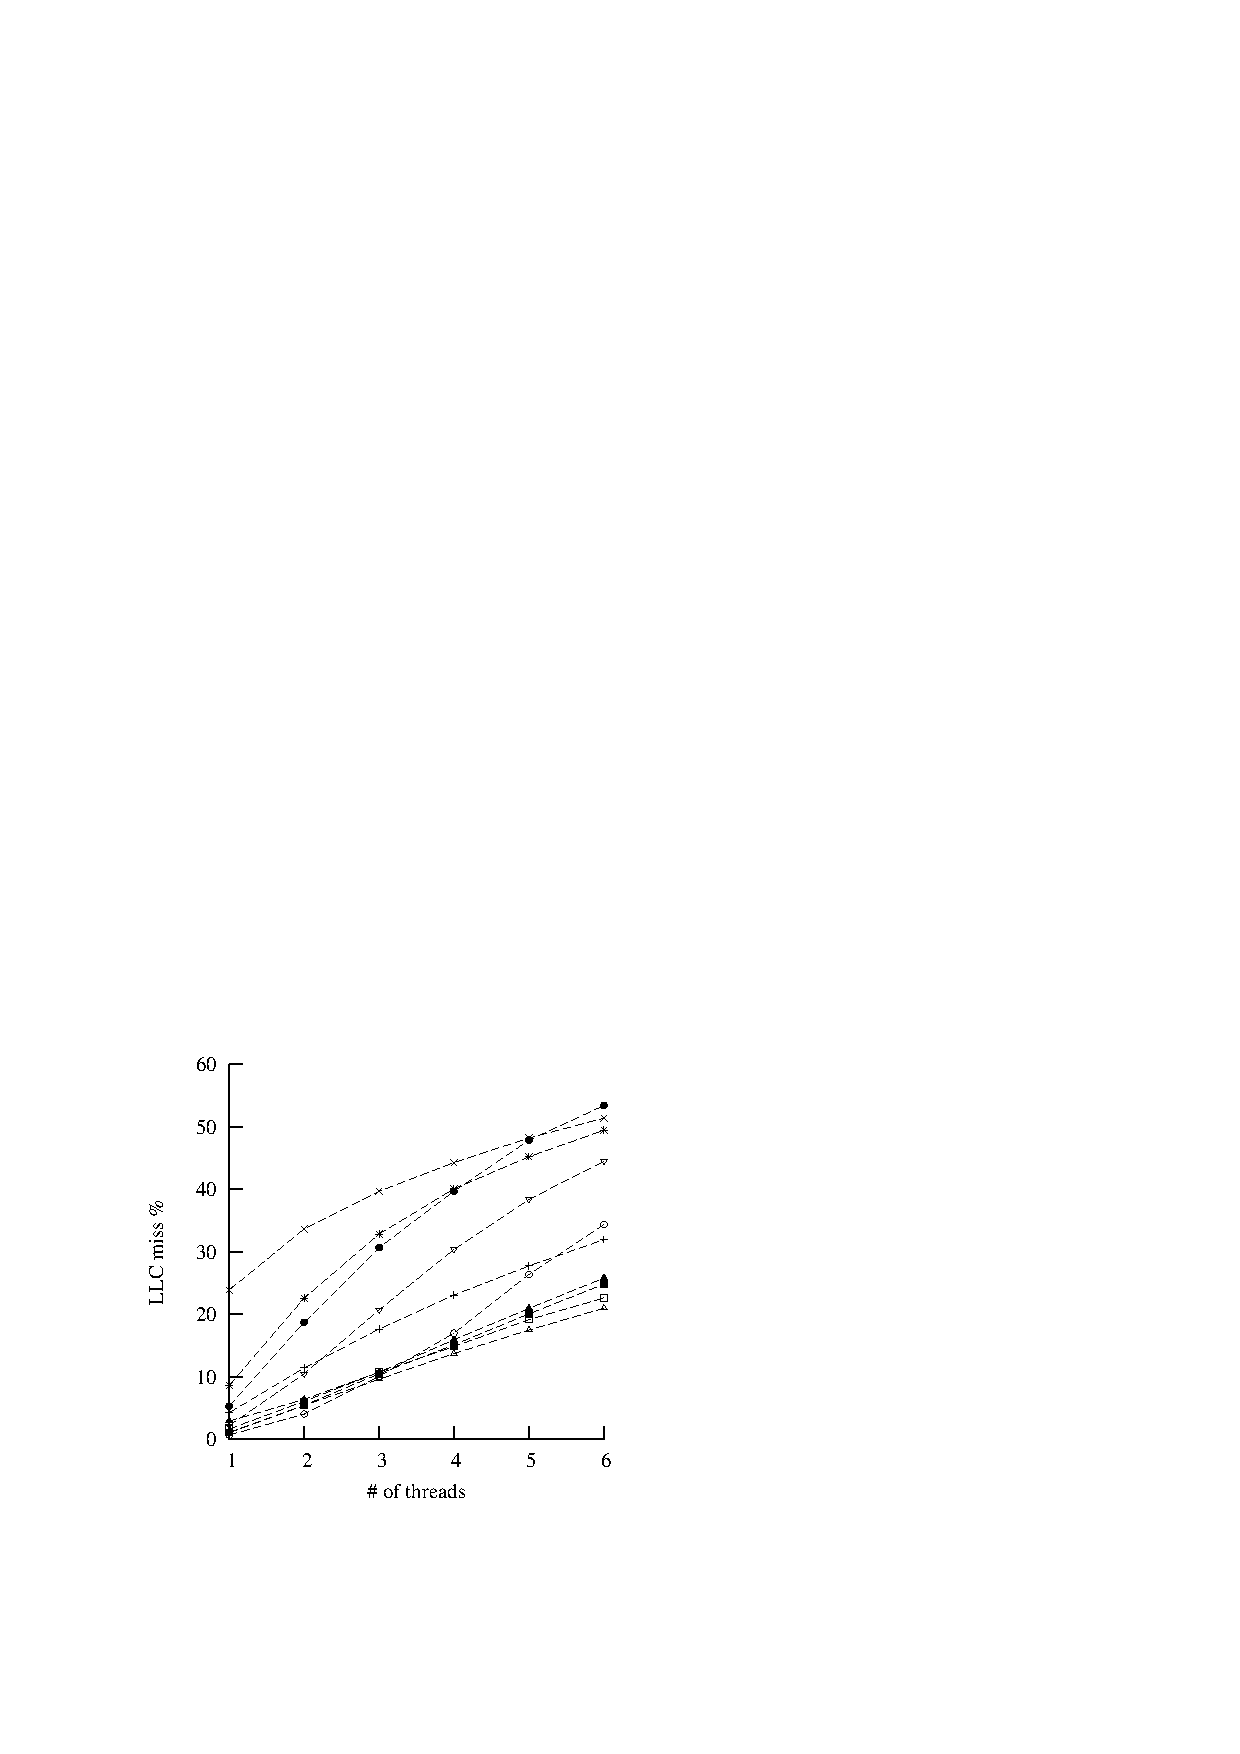
\includegraphics{plingeling_decay_cache}
  \caption{LLC statistics for modified \pling}
  \label{fig:LLCStats}  
\end{figure}

\subsection{\pling\ scalability}

In this section, we provide an overview of how \pling\ behaves at a
larger scale. So far, because of the experiment above, we know that
the more threads we add, the more cache hits/misses impacts negatively
in performance. However, we also know that adding threads also adds
new (and possibly successful) strategies. This results in a trade-off
between cache contention versus portfolio-approach benefits. To find
out where the trade-off equilibrium lies, we ran the original \pling\
over 207 standard benchmarks taken from past SAT races and
competitions (see link above), varying the number of threads from one
to ten on a single chip with 10 physical cores.

\begin{table}[hhh]
  \centering
  \begin{tabular}[h]{ccc}
    \hline
    {\bf Threads} & {\bf \# Problems solved} & {\bf Total time}\\
    \hline
    1&113&101399\\
    2&121&~95745\\
    3&119&~93854\\
    4&122&~90412\\
    5&124&~87953\\
    6&124&~89506\\
    7&127&~87416\\
    8&124&~88434\\
    9&124&~88931\\
    10&125&~89003\\
    10 in 4 CPUs & 129 & 85224\\
    40 in 4 CPUs & 123 & 92387\\
    \hline
    \hline
  \end{tabular}    
  \caption{Scalability}
  \label{tab:scal}
\end{table}


\begin{figure}[htp]
  \centering
  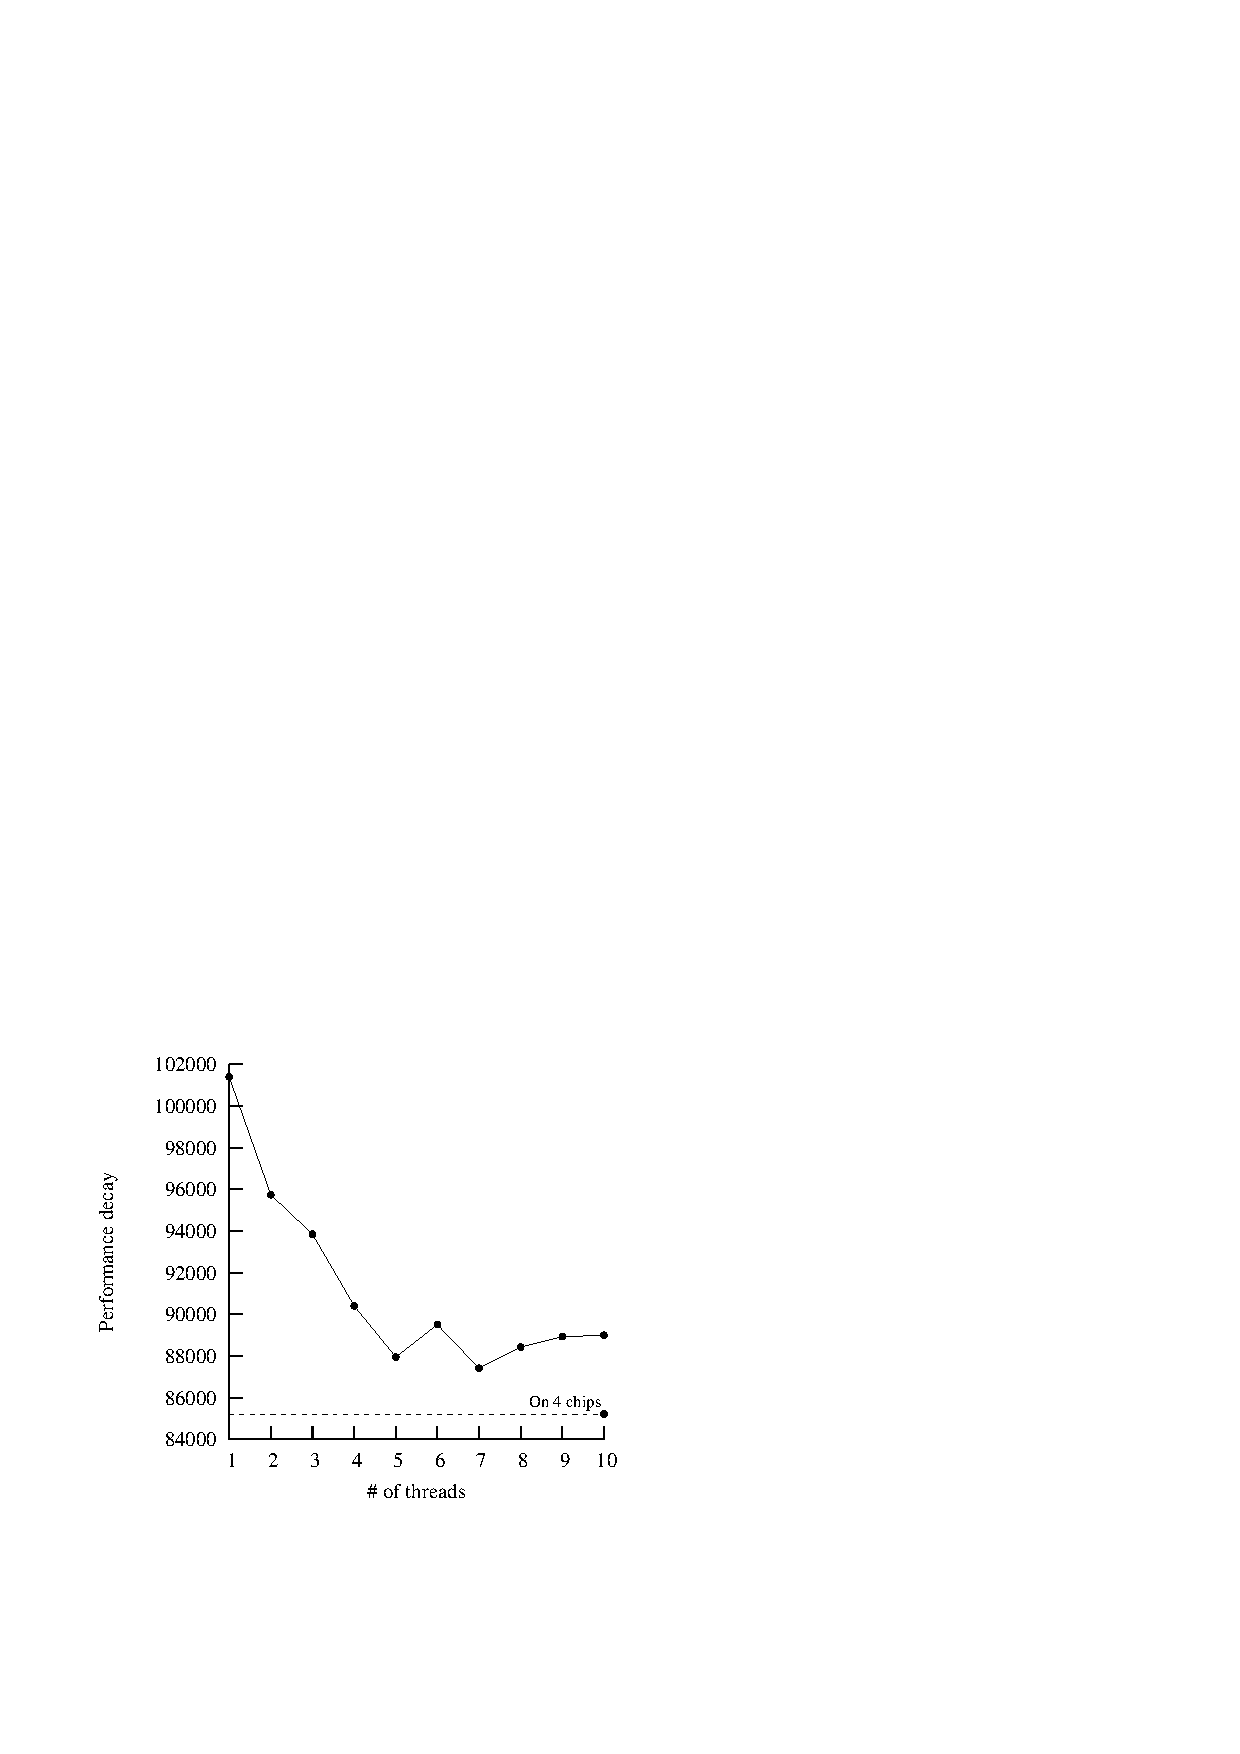
\includegraphics[scale=1]{plingeling_207_files}
  \caption{Total solving time per number of threads.}
  \label{fig:pperfpthread}
\end{figure}

Figure \ref{fig:pperfpthread} and Table \ref{tab:scal} show that up
until the fifth thread, scalability is good, but from then on, the
number of solved problems and total time reaches a plateau. This means
that \pling\ cannot scale up on the number of cores sharing an LLC. It
is important to notice that executing the same ten-thread solver in
four different physical CPU chips solves more problems in less time,
while executing a 40-thread solver (10 threads per chip) behaves worse
than the four-threaded single-chip version. This effectively means
that sharing cache among threads has a negative impact in the overall
behavior of modern portfolio-approach-based parallel SAT solvers.


%but it does scale on number of separate chips.

%%% Local Variables: 
%%% mode: latex
%%% TeX-master: "sat"
%%% End: 
